\documentclass[10pt]{sigplanconf}

%\ConferenceName{ACM ONWARD Papers 2015}
%\ConferenceShortName{ONWARD 2015}

%\usepackage{fullpage}
\usepackage{natbib}
\usepackage{breakurl}
\usepackage{algorithmic}
\usepackage{alltt}
\usepackage[ruled]{algorithm2e}
\usepackage[cmex10]{amsmath}
\usepackage{url} 
\usepackage{graphicx}
\usepackage{listings}
\usepackage{wrapfig}
\usepackage{multirow}
%\usepackage[plainpages=false, colorlinks=true, urlcolor={cyan}, citecolor={red}, linkcolor={green}]{hyperref}
\usepackage[plainpages=false]{hyperref}
\usepackage{array}
\usepackage{balance}
\usepackage{subfigure}
\usepackage{amssymb}
\usepackage{float}
\usepackage{caption}
\usepackage{placeins}

% % % % % % % % % % % % % % % % % % % % % % % % % % % % % % % % 
\lstset{frame=none, xleftmargin=15pt, stepnumber=1, numbers=left, numbersep=5pt,
numberstyle=\tiny, belowcaptionskip=\bigskipamount,
captionpos=b, escapeinside={*'}{'*}, language=java, tabsize=2, emphstyle={\bf},
commentstyle=\it, stringstyle=\mdseries\ttfamily, showspaces=false,
keywordstyle=\bfseries, morekeywords={in,do,print,Metadata,Where}, columns=flexible,
basicstyle=\footnotesize\ttfamily, showstringspaces=false, morecomment=[l], mathescape=true}



\newcommand{\solution}{\bigskip\hrule\bigskip}
\newcommand{\problembreak}{\bigskip\hrule\bigskip}

\renewcommand{\theenumi}{\bf\Alph{enumi}}

\newlength{\spread}
\setlength{\spread}{1.0in}

\def\bibfont{\footnotesize}

% correct bad hyphenation here
%\hyphenation{op-tical net-works semi-conduc-tor}


%%%%%%%%%%%%%%%%%%%%%%% END of LaTeX definitions %%%%%%%%%%%%%%%%%%%%%%%%%%%%

\begin{document}

\permissiontopublish
\conferenceinfo{ONWARD~'15}{October 25--30, 2015, Pittsburgh, Pennsylvania, USA} 
\copyrightyear{2015} 
\copyrightdata{978-1-4503-1995-9/13/10} 
\doi{2508075.2514879} 

\title{An Objective Assessment of Musical Complexity: Translating Music Pedagogy's Deep Insights with Novel Computing Paradigms}

\authorinfo{Ethan Holder}
					 {Software Innovations Lab at Virginia Tech}
					 {eholder0@vt.edu}
					 
\authorinfo{Eli Tilevich}
					 {Software Innovations Lab at Virginia Tech}
					 {tilevich@cs.vt.edu}
					 
\authorinfo{Amy Gillick}
					 {Department of Music at Virginia Tech}
					 {agillick@vt.edu}

\maketitle



\begin{abstract}

In the Western classical tradition, musicians play music from notated sheet music, called a score. When playing music from a score, a musician translates its visual symbols into sequences of instrument- specific physical motions. Hence, a music score's overall complexity represents a sum of the mental and mechanical acuity required for its performance.

Musicians often debate and disagree about the relative complexity of music scores, while the ability to accurately assess a score's complexity is required for curricular recommendations, competition specifications, etc. Unfortunately, this non-trivial cognitive task depends solely on individual opinions, a process influenced by personal biases and lacking common criteria. Additionally, people buying sheet music face great uncertainty when determining whether unfamiliar music matches their playing ability. With combined expertise from the fields of Computer Science and Music Pedagogy, this project finally offers an objective solution to these debates.

At the technical level, this interdisciplinary research exploits a fundamental musical tenet that—for a given instrument—different notes, intervals, and key signatures represent dissimilar levels of difficulty, which vary depending on the performer's proficiency. Tempo, dynamics, and articulation also affect the overall difficulty. We have realized our approach as a two-phase process. First, music experts rank the relative difficulty of musical components for different playing proficiencies and instruments. Second, an automated algorithm applies this ranking to music scores and calculates their respective complexity. Once music experts agree upon the complexity ranking for a given level of proficiency, our approach automatically calculates a music score's relative difficulty. The results of this interdisciplinary research project will empower musicians to expeditiously assess a music score's suitability for the abilities of intended performers.

This project is the first attempt to create a systematic and objective approach to assessing the complexity of a music score. The approach leverages computing technologies to be able to automatically and accurately calculate the complexity of playing a music score on a given instrument. As a proof-of- concept of the approach, we have been developing an automated, Web-based application for music educators and performers. This interdisciplinary research creates novel computing paradigms that systematically translate deep insights of Music Pedagogy, benefiting a broad music audience. Although the end product of this research will largely benefit musicians, the created novel computing concepts and paradigms will enhance the state of the art in computing, being applicable to solving important problems in other domains.

\end{abstract}

%\category{D.2.2}{Software Engineering}{Design Tools and Techniques}[Evolutionary prototyping \and Computer-aided software engineering (CASE)]
\keywords{Software; Software Engineering; Music; Translation; Assessment; Scoring; MusicXML; Java; Javascript


\section{Introduction} 
\label{sec:intro}

Briefly lead into the following subsections.

\subsection{Background} 
\label{sec:background}

Provide an overview of music concepts, what they mean, how they impact play, and generally define our terms for the remainder of the paper. This could also probably stand alone after the abstract as its own section depending on its size. We'll need to be careful not to let this cover too much space even though we'll need to cover a lot of information.

\begin{figure}[ht!]
	\centering
		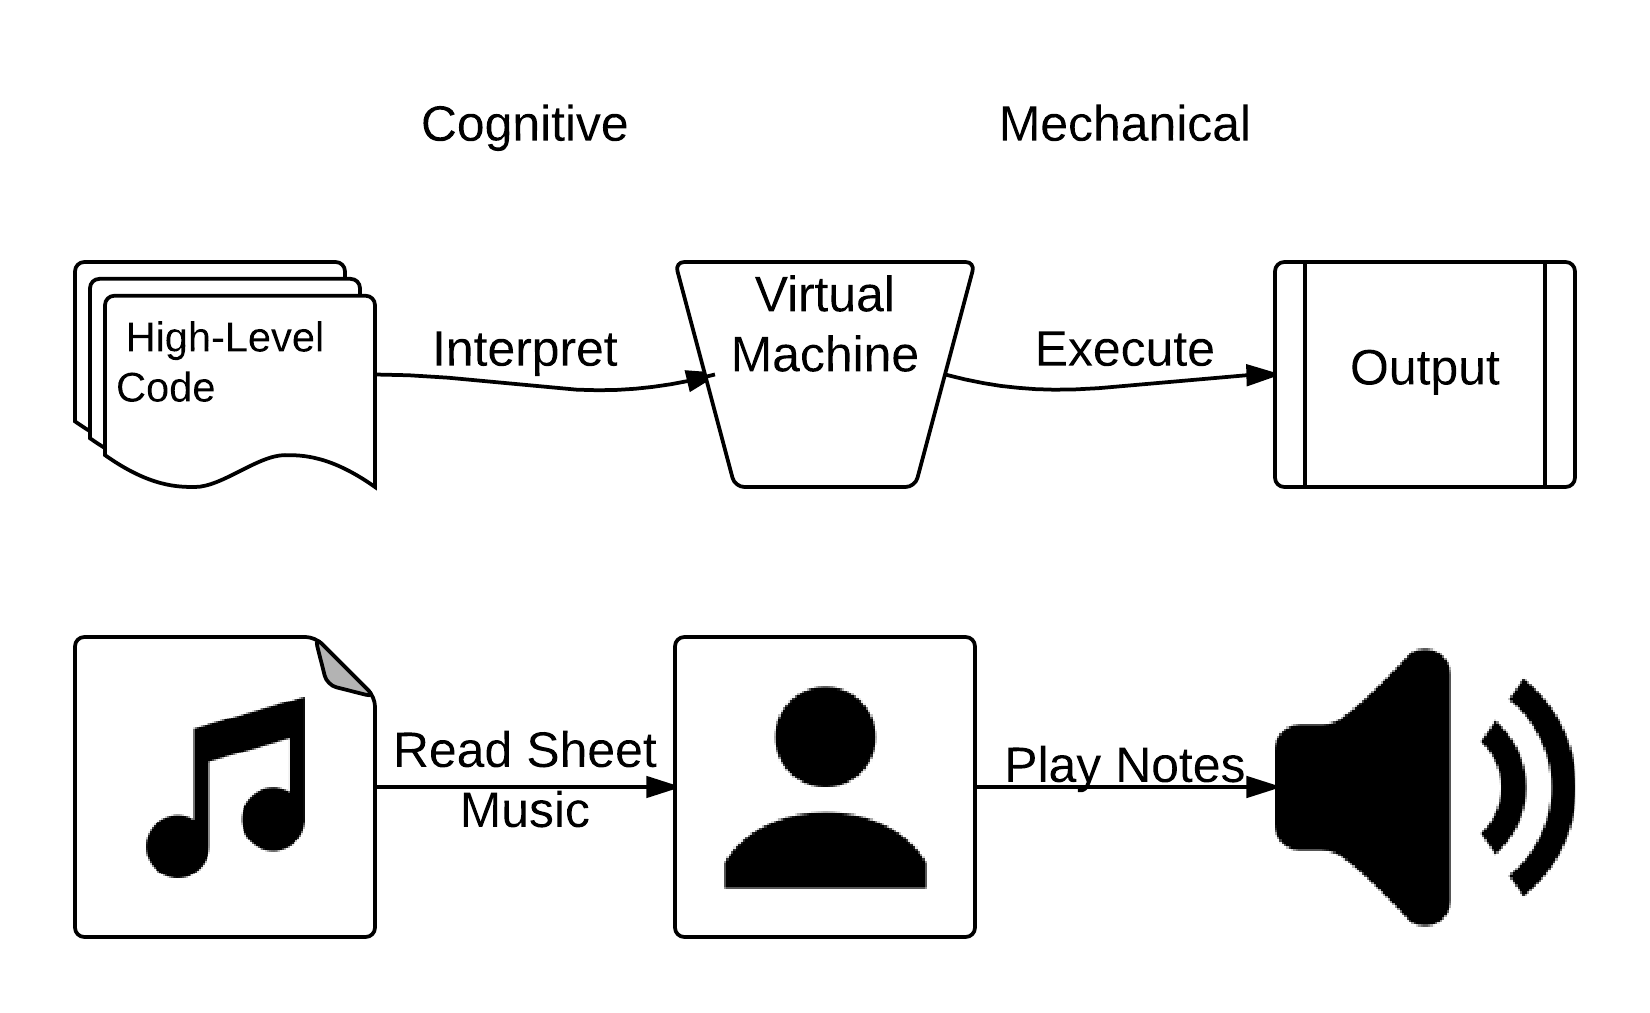
\includegraphics[width=0.47\textwidth]{CognitiveMechanical.png}
		\caption{The process of playing music introduces cognitive and mechanical complexities in interpreting written notes and creating a sound, respectively.}
		\label{image:complexities}
\end{figure}

\subsection{Motivation} 
\label{sec:motiv}

Move the motivating parts from the abstract down to here and make it flow together. This should flow naturally out of the background and abstract to present the general problem in the current state of the art.

\subsection{Research Questions/Goals} 
\label{sec:rqg}

Concretely define exactly what our goal is for this paper. This should naturally flow out of the motivation section.

\subsection{Paper Layout} 
\label{sec:layout}

The remainder of this paper is structured as follows. First, related work in this field is highlighted in \ref{sec:related}. Next, we explain the implementation of our scoring system in \ref{sec:imple}. This leads into the experimental setup section which shows how the current difficulty settings in \ref{sec:experiment}. The results in \ref{sec:results} then show exactly what we have uncovered through the implementation and user experiments so far. The analysis follows after the results and discusses how our system compares to others in the wild \ref{sec:analysis}. Next, brief directions for future work are given in \ref{sec:future}. Finally, we present our conclusions for this project in \ref{sec:conclu}.

\section{Related Work} 
\label{sec:related}

Cover any related work in the field and differentiate this project.

\section{Implementation} 
\label{sec:imple}

Cover first the overall design of the project and drill down to the deeper implementation details.

\subsection{Design Overview} 
\label{sec:design}

Talk about the high level approach for how this works in terms of the musical elements defined in the background section earlier.

\subsection{Code Details} 
\label{sec:details}

Very briefly talk about the actual implementation details. This should not span more than a paragraph or two just talking about the lines of code written, the libraries used, and the languages utilized.

The source code for this project is available for public consumption on github \footnote{\url{https://github.com/xwsxethan/MusicScoring}} \cite{GithubMusicScoring}.

\section{Experimental Setup} 
\label{sec:experiment}

Describe the preliminary settings used to score pieces based on clarinet and how we plan to refine them. Also talk about usability

\subsection{Clarinet Difficulty Settings} 
\label{sec:settings}

Explain what difficulty values and multipliers we came up with for clarinet and why.

\subsection{External Survey} 
\label{sec:survey}

Describe our methodology for surveying experts in the field and what questions we plan on asking them to refine our data. Also, mention the future work implications of surveying for other instruments.

\subsection{Usability} 
\label{sec:usability}

Talk about how the website is setup to be very user friendly and easy to navigate.

\section{Results} 
\label{sec:results}

Talk about our scores for various pieces and graph the results. We can talk about how it works for multiple parts, but we have to mention that the current settings are not meant for different instruments. Also cover any results we may have from the survey at that time (if any).

\section{Analysis} 
\label{sec:analysis}

Compare our results from objectively scoring to similar scoring methods by state school groups. Talk about the opportunities for this methodology to expand as well as its usefulness.

\section{Future Work} 
\label{sec:future}

Talk about the challenges we haven't addressed but want to next, like scaling the score range to between 1 and 100, joining this technology with imslp.org, leveraging SeeMore to show it off, and associating different part names to various instruments.

\section{Conclusions} 
\label{sec:conclu}

Sum up the paper.

\section*{Acknowledgements} 
\label{sec:ack}

Thank everyone and list any outside funding or support.




% The bibliography should be embedded for final submission.
\medskip
%\nocite{*}
%\bibliographystyle{abbrvnat}
\bibliography{HolderOnward2015}
\bibliographystyle{abbrv}


\end{document}
